% ----------------------------------------------------------
% Abordagem Teórica: Uma breve descrição que explique o 
% contexto teórico abordado pelo assunto.
% ----------------------------------------------------------

\chapter[Parte Prática]{Parte Prática}
%\addcontentsline{toc}{chapter}{Abordagem Teórica}
Em sala, montamos o circuito com base na esquemática da \autoref{figuras/fig3_CircuitoAula}.

\begin{figure}[htb]
  \caption{\label{figuras/fig3_CircuitoAula}Esquema de circuito com transistor como chave}
  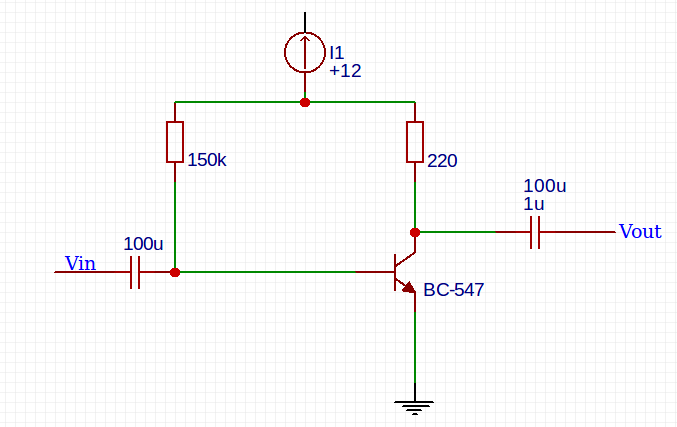
\includegraphics[scale=0.50]{figuras/fig3_CircuitoAula}
  \centering
\end{figure}

\section[Componentes e Equipamentos]{Componentes e Equipamentos} 

Abaixo os Componentes e equipamentos que foram utilizados nesta experiência:
\begin{itemize}
    \item 2x Capacitores de 100 $\mu$F
    \item 1x Resistor de 220 $\Omega$
    \item 1x Resistor de 150 k$\Omega$
    \item 1x Transistor BC547
    \item 1x Multímetro
    \item 1x Osciloscópio
    \item 1x Gerador de funções
    \item 1x Fonte de bancada
    \item 1x Protoboard
\end{itemize}


\section[Medições]{Medições}

\subsection{Tensões e Correntes}

As seguintes tensões foram medidas:

\par  $V_{CC}$= 12,00 V - $V_{RB}$= 11,44 V
\par  $V_{RC}$=  5,83 V - $V_{BE}$=  0,64 V 
\par  $V_{CE}$=  6,30 V - $V_{CE}$=  9,40 V 


Com esses valores aplicamos a lei de Ohm para calcular os valores das correntes, onde $V = R.I$:\\

$I_c=\frac{V_{RC}}{RC} = \frac{5,83}{220} = 26,5 mA$


$I_b=\frac{V_{RB}}{RB} = \frac{11,44}{150.10^3} = 0,076 mA$


$I_e= I_b + I_c = 26,576 mA$


\subsection[Gerador de Áudio]{Gerador de Áudio}

Para $f=1kHZ$, $V_{in}=0,1V_{pp}$, qual será o valor de $V_{out}$


Resposta:$0,1  V_{pp}$
\subsection{Valor máximo do sinal aplicado ao $V_{in}$}
Resposta: $8  V_{pp}$


% \section[Circuito]{Circuito}
% 
% Com os componentes citados no \autoref{Componentes e Equipamentos}, montamos o circuito abaixo:
% 
% \begin{figure}[htb]
%   \caption{\label{figuras/fig4_CircFinal}Circuito montado}
%   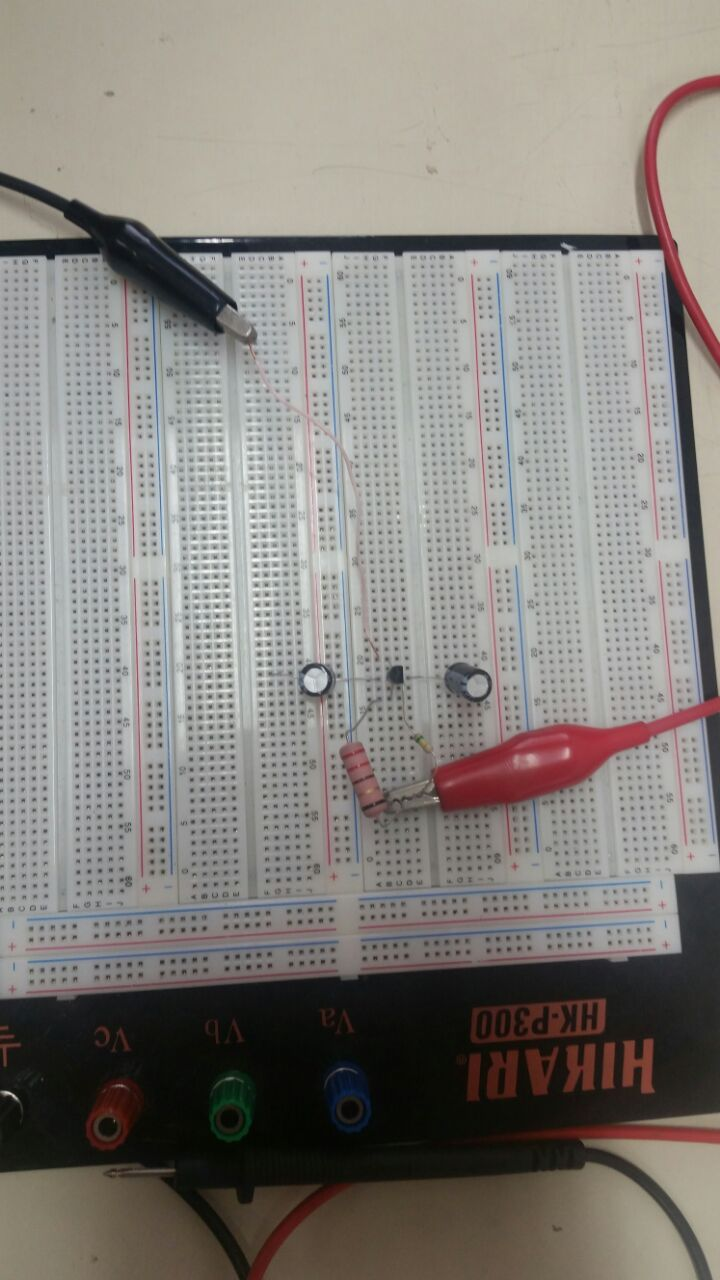
\includegraphics[scale=0.25]{figuras/fig4_CircFinal}
%   \centering
% \end{figure}